\section{Examples}
\subsection{K-Clustering}
\begin{frame}{K-Clustering}
  \begin{itemize}
    \item Simplest unsupervised learning algorithm that solve the clustering problem.
    \item The process by objects are classified into number of groups ensuring they are as much dissimilar from one group to the other, and as much similar within each group.
    \item Grouping is done in the following fashion:
          \begin{itemize}
            \item Determine the centroid co-ordinate for each cluster
            \item Calculate the Euclidean distance from each object to the centroid of the cluster
            \item Group the object based on minimum distance
          \end{itemize}
  \end{itemize}
\end{frame}

\begin{frame}{K-Clustering}
	Conflict in K-Clustering algorithm
			\begin{figure}
			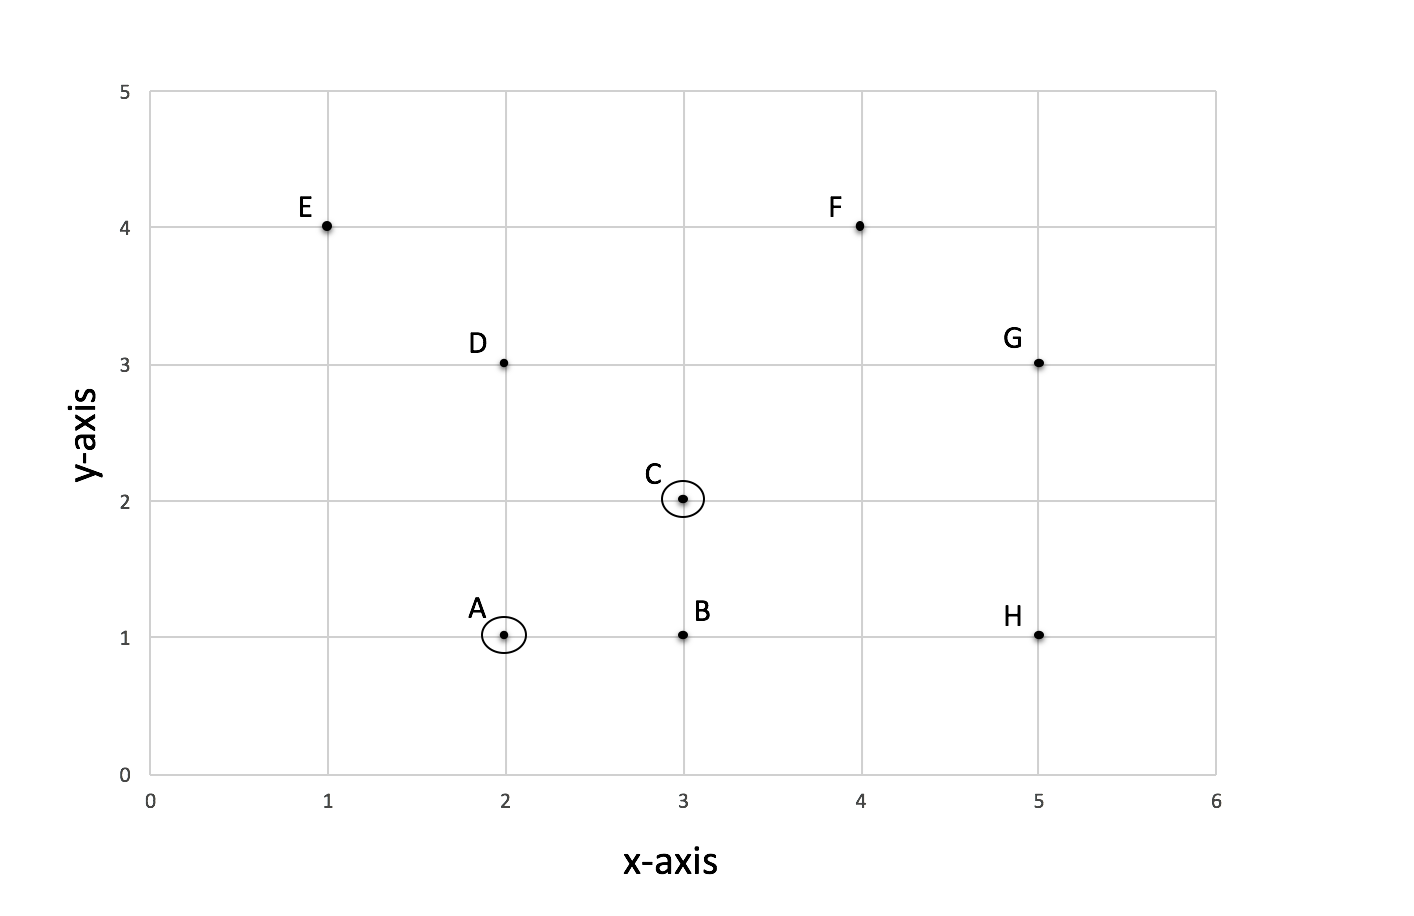
\includegraphics[width=0.8\linewidth]{figures/k-cluster.jpg}
			\caption{K-Clustering algorithm}
			\end{figure}
\end{frame}

\begin{frame}{K-Clustering}
  Co-ordinates of data points:
  \newline
  \newline
  A=(2,1), B=(3,1), C=(3,2), D=(1,2),\\
  E=(1,0), F=(4,4), G=(5,3), H=(5,1)
  \newline
  \newline
  where $B, D, E, F, G, H$ are data points\\
  $A$ and $C$ are two clusters\\
\end{frame}

\subsection{Synthesized Example}
\begin{frame}[fragile]
\begin{lstlisting}[
    language=Java]
  Public class SimpleMutateGraphComputation extends BasicComputation<
    LongWritable, DoubleWritable, FloatWritable, DoubleWritable> {

    public void compute(Vertex<LongWritable, DoubleWritable, FloatWritable>
      vertex, Iterable<DoubleWritable> messages){
      if (getSuperstep() == 0) {
        if(vertex.getID() == getVertexCount()-1)
          removeVertexRequest(getVertexCount());
        else
          addEdgeRequest(getVertexCount()-1, vertex.getID());
      } else if (getSuperstep() == 1) {
        vertex.voteToHalt();
    }
  }
\end{lstlisting}
Example of a dangling edge conflict
\end{frame}
